In this Chapter, we conducted 4 different experiments in simple maze environments to investigate how the ILP(RL) agent learns and reaches the optimal policy.

\section{Experimental Setup}
\label{sec:experimental_setup}

\subsection{Evaluation Metrics}
\label{subsec:evaluation_metrics}

As introduced in \ref{sec:motivation}, our motivation is to improve the RL learning efficiency and capability of transfer learning.
Therefore, these are the two main measurements for the performance of ILP(RL).

The learning efficiencies are measured in two different ways. First, the performance of ILP(RL) is compared with benchmarks in terms of
convergence rate, which is measured in terms of the number of episodes that the agent requires to get to an optimal policy.
The optimal policy can be measured in terms of the total reward that the agent gains at each episode. 
Throughout the experiments, we designed the environment such that the agent receives reward of -1 for any state except the terminal state, and receives reward of +10 for the terminal state, or the goal.
For example, if the agent needs the shortest 10 actions to get to the terminal state, the maximum reward the agent could get per episode is 0 (-1 reward at each action + 10 for reaching the goal).
We log the rewards at each time step and calculate the total reward at each episode. 
Since the agent follows an random exploration throughout the learning, the total reward never converges to the maximum in learining. 
Therefore at each episode, we also measure the performance without exploration to see the pure optimal policy.

Second, the convergence of learning by ILASP is measured to see the learning curve of ILP(RL), which is defined as follows:
\begin{equation}
\begin{split}
\frac{\textsf{The cumulative number of ILASP calls per time step at episode 0}}{\textsf{The total number of ILASP calls in all episodes}}
\end{split}
\end{equation}
The reason we are measuring it only at episode 0 is that empirically the agent learns most of the target hypotheses within episode 0 and there is no hypothesis refinement after episode 0.
This gives a normalised convergence rate of ILASP learning with the maximum 1, and we plot it across each time steps. 
If an indutive learning happens after episode 0, this included in the deniminator, and the maximum convergence plot is strictly less than 1.

RUNTIME

\subsection{Benchmarks}
\label{subsec:benchmarks}
We use different benchmarks for learning evaluation and transfer learning evaluation. 

For learning evaluation, we use two existing RL methods as benchmarks: Q-learning and tile-coding.
Q-learning is widely used RL technique, and given the environments used for the experiments are discrete and deterministic, this method is sufficient for our experiments.
XX the Q-values are initialised as XX. (Optimistic and pessimistic initialisation.)

Another benchmark is tile coding, which is a type of linear function approximation techniques described in Chapter XX.
The reason for using an extra benchmark is that the performance comparision of ILP(RL) with q-learning might not be a fair comparision,
since ILP(RL) has one extra assumption: the agent knows surrounding information (whether there are walls in adjacent cells),
which is not a common assumption for Q-learning. Thus we incorporate the same surrounding information as features, and update the weights of each feature as a learning.
We compare the performance of ILP(RL) with these two methods.

% \textcolor{red}{TODO Details of tile-coding configuration}
For transfer learnig evaluation, 

\subsection{Parameters}
\begin{table}[!ht!b]
\centering
\begin{tabular}{lll}
\hline
Parameter            & ILP(RL)    & Benchmarks      \\ \hline
The number of episode& 100        & 100        \\
Time steps per episode& 250        & 250        \\
The number of experiments& 30       & 30       \\
% Discount rate        & 0,5       & 1.4e-2       \\
Alpha                & N/A       & 0.5       \\
Epsilon              & 0.1        & 0.1        \\
\end{tabular}
\caption{List of parameters used in the experiments}
\label{param}
\end{table}

Agents are trained in 250 time steps with 100 episodes, and conducted the same experiment 30 times in each environment. 
The resulting average score is plotted for each experiment.
All the matrices used in the experiments are summarised in Table \ref{param}.
The number of episode is set such that both the benchmarks as well as ILP(RL) eventually eaches the optimal policy. 
The number of time steps should be sufficient for the both algorithms to reach the terminal state by the random exploration, 
which we set 250 time steps for all experiments. If the agent does not find the terminal state by 250 time steps, the agent receives the reward of -250 and 
start the next episode from the starting point. If the agent reaches the terminal state within 250 time steps, it receives the reward of 10 and start the next episode with the same starting point. 

Starting point is fixed every episode. 
% Epsilon for ILP(RL) should be higher, since the agent follows the generated plan,
% whereas benchmark algorithms update value function with the degree of alpha.
We conducted several experiments using different environments to highlight each aspect of the algorithm.

Each experiment is conducted 30 times and the perform is averaged across the experiments, 
since the performance of the agent is affected by the randomness of the exploration,
and ILP(RL) is highly dependent on how quickly the agent finds the goal.

\section{Learning Evaluation}
\label{sec:learning_evaluation}

\subsection{Experiment 1: Setup}
\label{subsec:experiement1_setup}

\begin{figure}[!htb]
\centering
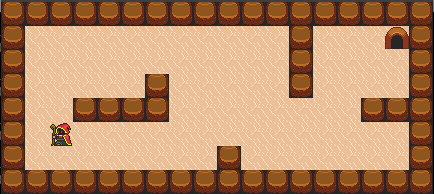
\includegraphics[width=0.5\textwidth]{./figures/experiment1}
\caption{Game environment for experiment 1}
\label{fig:experiment1}
\end{figure}
    
The purpose of the first experiment is to highlight how ILP(RL) agent learns hypotheses in ILASP.
The environment are designed as a simple maze where the terminal state is located the right uppper corner as shown in Figure \ref{fig:experiment1}.

The agent's starting location is the same at every episodes. The agent's goal is to learn hypotheses for valid move of the game, and to use the hypotheses to correctly plan a sequence of actions to reach the goal.
The shortest path between the agent's starting point and the terminal state is 18 steps, thus the maximum total reward the agent could gain is -8.
    
\subsection{Experiment 1: Result}
\label{subsec:experiment1_result}

\begin{figure}[!htb]
\centerline{
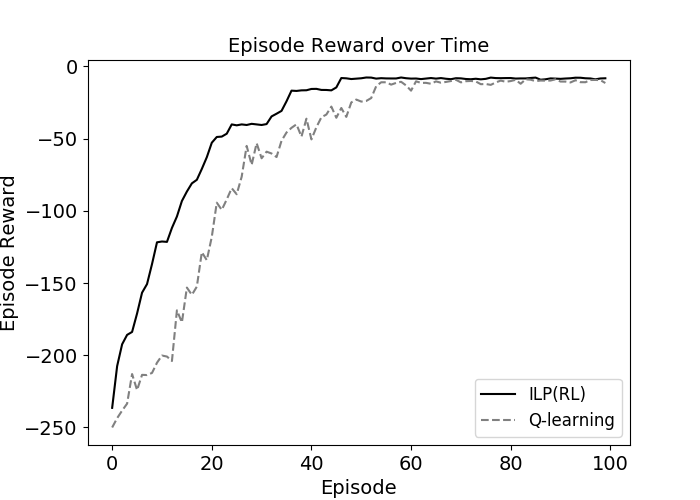
\includegraphics[width=0.55\textwidth]{./figures/experiment1_training}
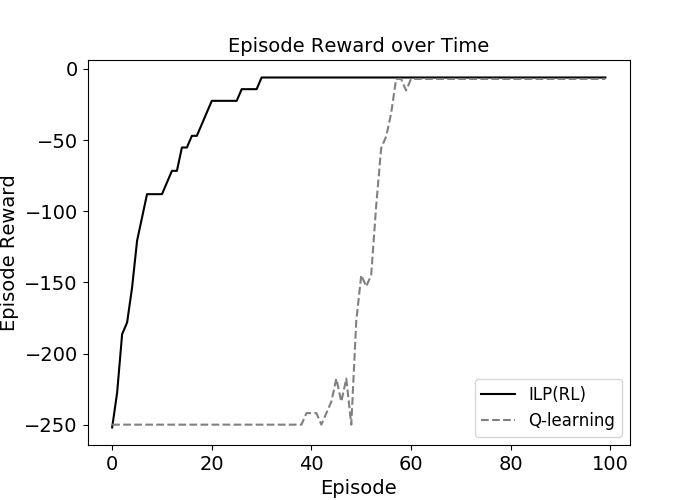
\includegraphics[width=0.55\textwidth]{./figures/experiment1_test}
}
\caption{Results of experiment 1: learning curve (left) and testing (right)}
\label{experiment1_result}
\end{figure}

Figure \ref{experiment1_result} shows the traning performance between ILP(RL) and Q-learning.
The convergence rate of ILP(RL) is faster than Q-learning: ILP(RL) reaches the maximum reward between 40 and 50 episodes, whereas Q-learning reaches the same level at between 60 and 70 episodes.
This is because unlike Q-learning where the value function is updated with the rate of alpha, ILP(RL) gradually builds the model of the environment and use the background knowledge to accurately plan.
This result is also consistent with the general notion that model-based RL is more data-efficient than model-free RL.
The same trend is also shown in Figure \ref{experiment1_test}, where we measure only the performance of the policy without random exploration.
The reason Q-learning converges slower in the testing than that of training is that Q values are initialised to 0, which means that XXX.
Overall this results shows that ILP(RL) converges to the optimal policy faster than benchmarks in a simple scenarios, achieving more data-efficient learning.

\lstinputlisting[
%   language = Prolog,
  caption  = {Hypotheses for experiment 1},
]{experiment1_hypothesis.pl}

% \lstinputlisting[
% %   language = Prolog,
%   caption  = {Anser sets for experiment 1},
% ]{experiment1_asp.pl}

In addition to the data-efficient learning, what the agent has learnt with ILP(RL) is expressive.
Learnt hypotheses are shown in \ref{experiment1_hypothesis}, which is the rule of the game and easy to understand for human users.
Since the learnt hypothesis is a general concept, which can be used in a different environmet.
This transfer learning capability is also described in Experiement 3 and 4.

Next, we see how the agent learns the hypotheses during over time. We plot the learning convergence for ILASP at episode 0 in Figure \ref{experiment1_ilasp}, measured in terms of the number of hypothesis refinement to reach the final hypothesis as shown in \ref{experiment1_hypothesis}.
This shows that the agent learns most of the hypotheses at the episode 0.
Since the two variables that the agent require to construct optimal answer set planning are the hypothese and background knowledge, in this case the location of the walls, 
the reason that the agent reaches the maximum reward at between 40 and 50 episodes, is mostly dependent on how quickly the agent finds the goal location.
Even though the agent acquires the full hypotheses at episode 0, without the terminal state, the agent continues to randomly explore the environment.
Since our exploration strategy is expilon random choice, there is a promissing that a better exploration strategy further accelerates the learning process.

\begin{figure}[!htb]
\centering
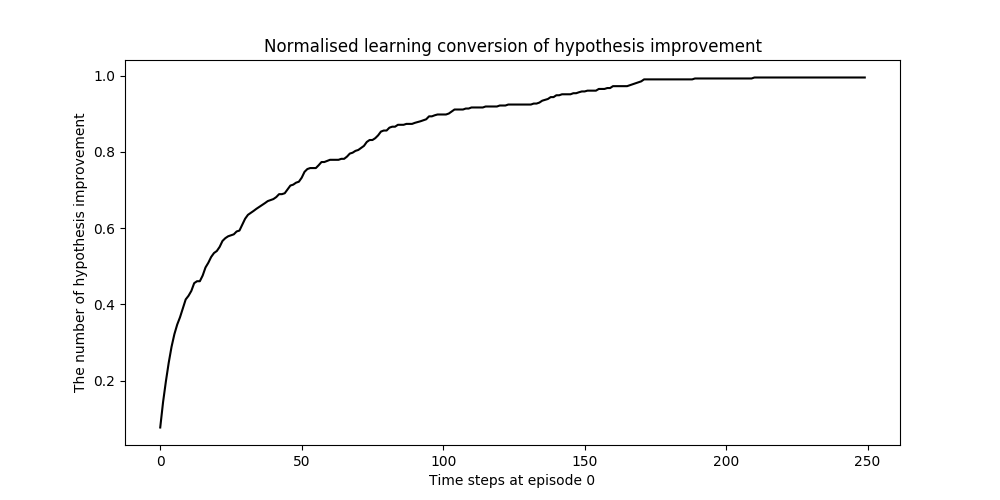
\includegraphics[width=0.9\textwidth]{./figures/experiment1_ilasp}
\caption{Normalised learning convergence by ILASP for experiment 1}
\label{experiment1_ilasp}
\end{figure}

Finally, we compare the runtime of two algorithms. 

This result confirms that inductive learning part is likely the bottleneck in terms of 

This issue may not be cretical in cases where the time between the time steps is not an issue. If the performace is measured in terms of computation time rather than the number of iterations, 
ILP(RL) is not likely to perform exisitng RL algorithms. 
The average runtime of inductive learning is 5.579 seconds, and there are on average 12.83 times inductive learning per episode. 
% RUNTIME FOR ILASP: 5.579039041812603
% ILASP RUNS TOTAL: 12.83 times
The plannning part is not a bottleneck of ILP(RL) compared to Q-leaning, but still takes longer time than Q-learning. While the planning with this environment is relatively simple planning. 
As discussed in XX, ASP also has its scalability issues. XXX

\begin{figure}[!htb]
\centering
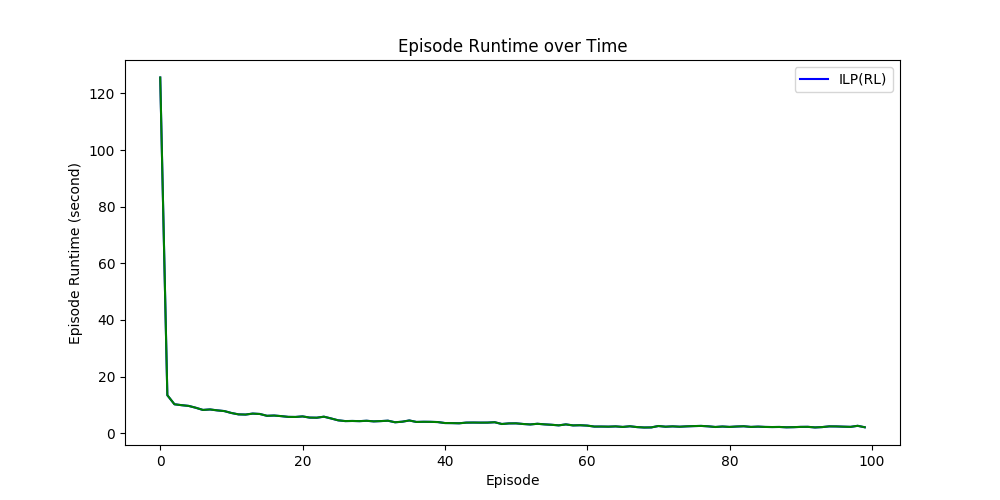
\includegraphics[width=0.9\textwidth]{./figures/experiment1_runtime}
\caption{Runtime comparision}
\label{experiment1}
\end{figure}

% \newpage

\subsection{Experiment 2: Setup}
\label{subsec:experiement2_setup}
\begin{figure}[!htb]
\centering
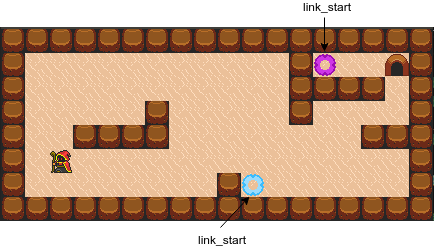
\includegraphics[width=0.5\textwidth]{./figures/experiment2_setup}
\caption{Game environment for experiment 2}
\label{experiment2}
\end{figure}
Experiment 2 was conducted to see if the agent find a optimal path of using a teleport. The environment is the same as experiment 1 except the presence of teleport link.
In the environment shown in Figure \ref{experiment3},
there are two ways to reach the goal: using a normal path to get the goal located on the top right corner, or using a telport.
The environment is designed such that using a teleport is a shorter path and therefore gives higher total reward.
Compared to Experiment 1, two extra search spaces and concepts are added as follows:
\begin{equation*}
\begin{split}
&\textsf{\#modeb(1, link\_start(var(cell)), (positive)).}\\
&\textsf{\#modeb(1, link\_dest(var(cell)), (positive)).}
\end{split}
\end{equation*}

Where teleport links are added to the environment. The teleport link is one-way: \textsf{link\_start} takes the agent to \textsf{link\_dest}, but \textsf{link\_dest} does not take the agent back to \textsf{link\_start}.
This extra types allows ILASP to learn additional hypothesis.
The full learning task for this experiment is in Appendix XX.

In VDGL game environmet, when the agent steps onto \textsf{link\_start}, it immediately takes the agent to \textsf{link\_dest}. This means that the agent moves two states in one time step.
Since our ASP translation part takes the state transition as \textsf{state\_before} and \textsf{state\_after}, 
we deal with this situation such that the agent receives two positive experiences in this time step rather than two time steps.

Also link\_start and link\_dest need to be stored in background knowledge rather than as contex examples,
because the framework need to generate exclusions regarding the link behaviour (TODO EXPLAIN MORE).
link locations need to be available for all positive examples so that ILASP correctly learn non-link for normal valid move rather than teleport, which is shown in Figure XX below.

Because of the teleport link, the shortest path is 13 steps to reach the terminal state. Thus the maximum total reward that the agent could gain is -3.

\subsection{Experiment 2: Result}
\label{subsec:experiment2_result}
% The game is designed such that
    
\begin{figure}[!htb]
\centerline{
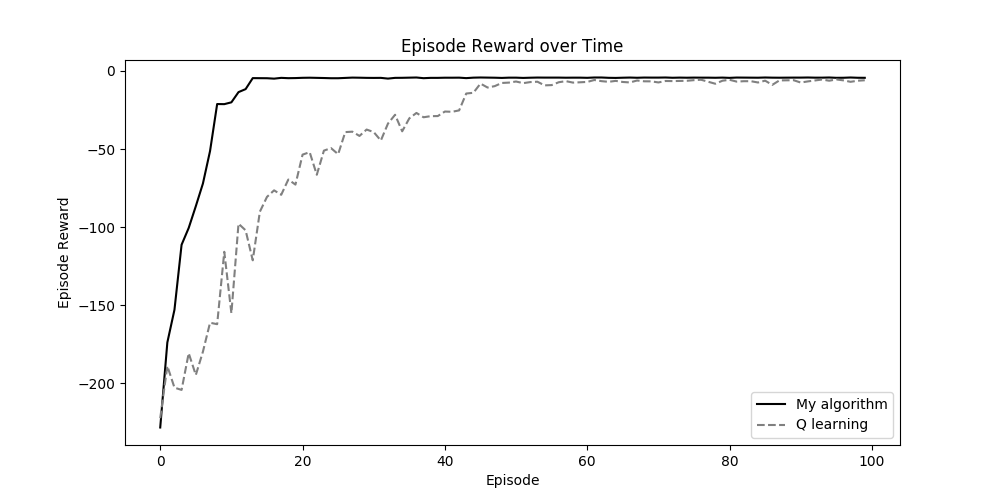
\includegraphics[width=0.55\textwidth]{./figures/experiment2_training}
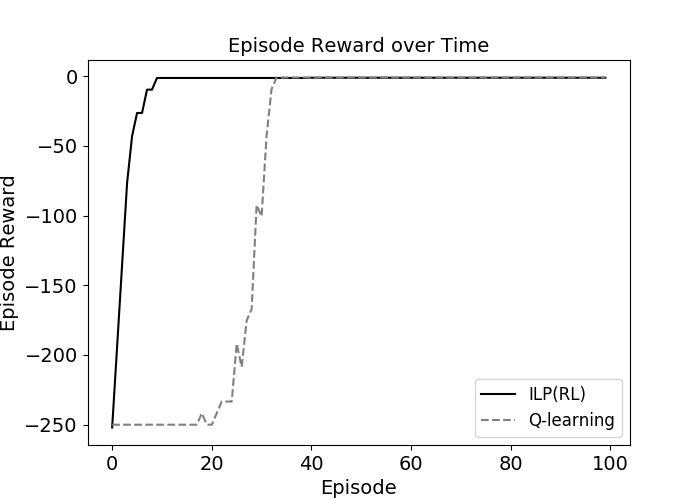
\includegraphics[width=0.55\textwidth]{./figures/experiment2_test}
}
\caption{Results of experiment 3: learning curve (left) and testing (right)}
\label{experiment2_training}
\end{figure}

The same as the Experiment 1, both training and test performance converges faster than that of Q-learning.

\lstinputlisting[
  caption  = {Incomplete hypotheses for experiment 2},
]{experiment2_hypothesis_intermediate.pl}

% \begin{equation}
% \begin{split}
% &\textsf{state\_after(V1) :- link\_dest(V1).}\\
% &\textsf{state\_after(V0) :- link\_dest(V0), state\_before(V0), action(right).}\\
% &\textsf{state\_after(V1) :- adjacent(left, V0, V1), state\_before(V0), action(right), not wall(V1).}\\
% &\textsf{state\_after(V0) :- adjacent(left, V0, V1), state\_before(V1), action(left), not wall(V0).}\\
% &\textsf{state\_after(V1) :- adjacent(up, V0, V1), state\_before(V0), action(down), not wall(V1).}\\
% &\textsf{state\_after(V0) :- adjacent(up, V0, V1), state\_before(V1), action(up), not wall(V0).}\\
% &\textsf{state\_after(V1) :- adjacent(left, V0, V1), state\_before(V1), action(left), wall(V0).}\\
% &\textsf{state\_after(V1) :- adjacent(down, V0, V1), state\_before(V1), action(down), wall(V0).}\\
% &\textsf{state\_after(V1) :- adjacent(up, V0, V1), state\_before(V1), action(up), wall(V0).}
% \end{split}
% \label{experiment2_ilasp_imcomplete}
% \end{equation}

To highlight the learning process of the new concept of teleport link, Figure \ref{experiment2_ilasp_imcomplete} is an intermediate incomplete hypothesis learnt by ILASP.
These hypotheses are generated just after the agent steps onto the \textsf{link\_start}. However, the first hypothesis says
when link\_dest is available state\_after is true. Since link\_dest is available in background knowledge rather than context,
when solving for answer sets to generate a plan, it generates incorrect state\_after at every time step.

However, as shown in Algorithms XX, these generated state\_after are all incorrect and therefore will be added to exclusions of the next positive examples.
These exclusions will later refines hypotheses and results in Figure \ref{experiment2_ilasp_complete}, the final complete hypotheses.

Learnt hypotheses are shown in Figure \ref{hello}:

\lstinputlisting[
  caption  = {Complete hypotheses for experiment 2},
]{experiment2_hypothesis.pl}

% \begin{equation}
% \begin{split}
% &\textsf{state\_after(V1) :- link\_start(V0), link\_dest(V1), state\_before(V0).}\\
% &\textsf{state\_after(V0) :- link\_dest(V0), state\_before(V0), action(right).}\\
% &\textsf{state\_after(V1) :- adjacent(left, V0, V1), state\_before(V0), action(right), not wall(V1).}\\
% &\textsf{state\_after(V0) :- adjacent(left, V0, V1), state\_before(V1), action(left), not wall(V0).}\\
% &\textsf{state\_after(V1) :- adjacent(up, V0, V1), state\_before(V0), action(down), not wall(V1).}\\
% &\textsf{state\_after(V0) :- adjacent(up, V0, V1), state\_before(V1), action(up), not wall(V0).}\\
% &\textsf{state\_after(V1) :- adjacent(left, V0, V1), state\_before(V1), action(left), wall(V0).}\\
% &\textsf{state\_after(V1) :- adjacent(down, V0, V1), state\_before(V1), action(down), wall(V0).}\\
% &\textsf{state\_after(V1) :- adjacent(up, V0, V1), state\_before(V1), action(up), wall(V0).}
% \end{split}
% \label{experiment2_ilasp_complete}
% \end{equation}

Compared to the Experiment 1, there are two new hypotheses due to the presence of the teleport links.
These learnt hypotheses are also applicables to an environment where there is no link, such as a game in experiment 1.
In this case, the first two hypotheses in Figure XX are never be used since the body predicates relating to link\_start(V0), link\_dest(V1) are never be satisfied.
% RUNTIME AVERAGE: 95.47274640401204
% RUNTIME COUNTS: 16.233333333333334

Figure \ref{experiment2_ilasp} shows the learning convergence of inductive learning at episode 0.
Similar to Experiment 1, most of inductive learning occur at the beginning of the episode, as shown in Figure \ref{experiment2_runtime}. 
This result confirms that the agent learns inductive learnig at the beginning of episode.

Despite the fact that the size of the environment is the same as Experiment 1, 
there is a significant increase of runtime at the beginning of episode. This is because of the increase of search space as we added extra language bias.

There are increase of runtime after episode 0.
This is due to the fact that the agent later discovers a teleport link, which is a new hypothesis to be learnt. 
\textcolor{red}{TODO is this really true??}
The average runtime of inductive learning is 95.47 seconds, and there are on average 16.23 times inductive learning per episode.

\begin{table}[!ht!b]
\centering
\begin{tabular}{lll}
\hline
Parameter            & ILP(RL)    & Benchmarks      \\ \hline
Runtime per episode (seconds) & 95.47        & 1        \\
Average ILASP time (seconds)& XXX        & N/A        \\
The number of ILASP calls &  16.23      & N/A       \\
Hypothesis space &  XXX      & N/A       \\
\end{tabular}
\caption{Comparision of runtime}
\label{param}
\end{table}

While ILP(RL) still learns faster than Q-learning in terms of the number of iterations, 
the result of Experiment 2 shows that, the learning time per episode increases with respect to the size of search space, 
which corresponds to the number of symbolic representations that the agent needs to learn in the environment.

\begin{figure}[!htb]
\centering
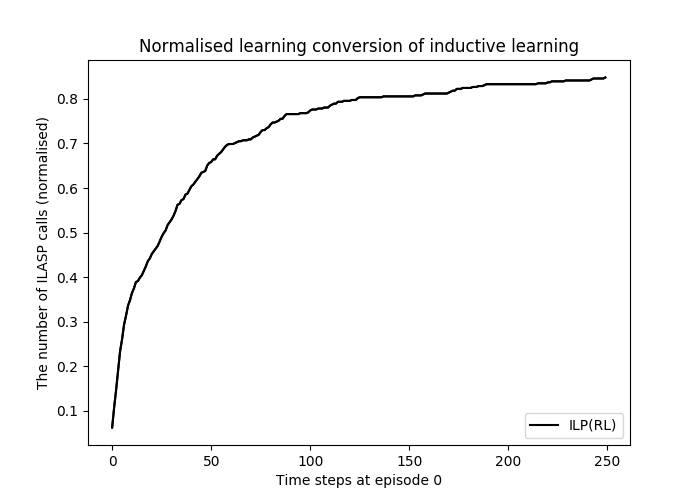
\includegraphics[width=0.55\textwidth]{./figures/experiment2_ilasp}
\caption{Normalised learning convergence by ILASP for experiment 2}
\label{experiment2_ilasp}
\end{figure}

\begin{figure}[!htb]
\centering
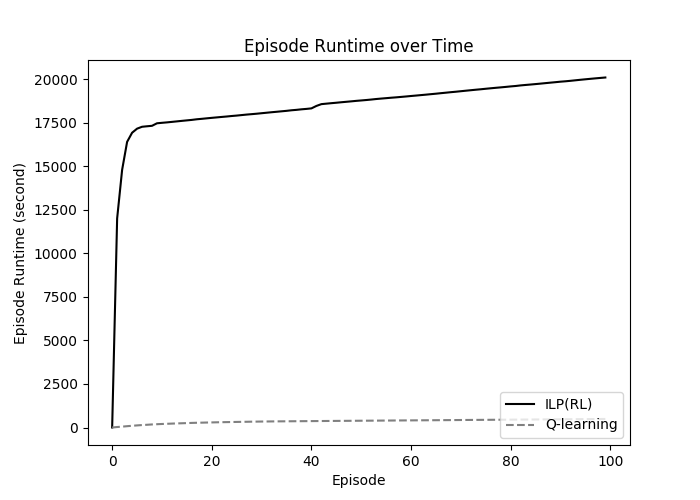
\includegraphics[width=0.55\textwidth]{./figures/experiment2_runtime}
\caption{Runtime comparision}
\label{experiment2_runtime}
\end{figure}

\clearpage
\newpage
\section{Transfer Learning Evaluation}
\label{sec:transfer_learning_evaluation}

\subsection{Experiment 3: Setup}
\label{subsec:experiement3_setup}

\begin{figure}[!htb]
\centerline{
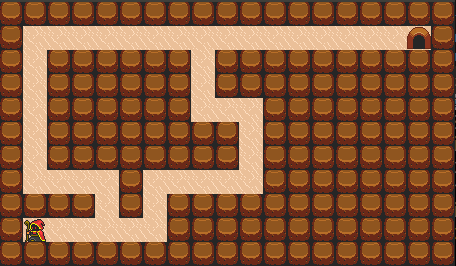
\includegraphics[width=0.5\textwidth]{./figures/experiment3_before}
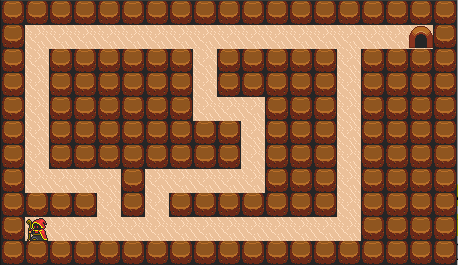
\includegraphics[width=0.5\textwidth]{./figures/experiment3_after}
}
\caption{Game environment for experiment 3: before (left) and after (right) transfer learning}
\label{experiment3_setup}
\end{figure}

In Experiment 3, we investigated the possibilites of transfer learning betweeen similar environments.
We trained the agent using the environment on the left in Figure \ref{experiment4}, and transfer the learnt hypothesis as well as positive examples to a new environment on the right in Figure \ref{experiment4}
The learnt hypothesis is valid move of the game and a general concept that is applicable to any similar environments. Positive examples are also transferred since
if there is a new hypothesis that the agent needs to learn in a new environment, the agent needs to refine the hypothesis by running ILASP in the new environment.
Thus the all the positice examples are also transferred as well as learnt hypotheses. 
Background knowledge are not transferred since the wall locations are different in a new environment.
The agent therefore starts the exploration of the new environment with an empty background knowledge and gradually collects them over time.
The goal position is the same as in the first game, but the shortest path to the goal is different between the two environments as new shorter path is introduced in the right environment in Figure \ref{experiment3_setup}.

We use four different agents as follows. 

\begin{itemize}
    \item Agent(TL): The agent with transferred hypotheses, examples and also remembers the location of the terminal state.
    \item Agent(noTL)\textsubscript{Goal}: The agent with transferred hypotheses, examples, but does not know the location of the terminal state.
    \item Agent(noTL)\textsubscript{noGoal}: The agent with no transferred information, neighther the hypotheses nor the location of the terminal state is known to the agent.
    \item Q-learning
\end{itemize}

While this is a limited transfer learning since the goal position is known in advance, this is still a useful transfer in cases where the terminal state is the same but the rest of the environment changes.

Figure XX is the hypotheses that is transferred to a new environment, which is acquired by training the agent in the environment once on the left of Figure \ref{experiment3_setup}.
The positive examples to be transferred are those the agent accumulated in the left environment, XXX examples in total.

\lstinputlisting[
%   language = Prolog,
  caption  = {Hypotheses for experiment 3},
]{experiment3_hypothesis.pl}

\subsection{Experiment Result 3}
The result is shown in Figure \ref{experiment3_training} and \ref{experiment3_test}.
For Agent(TL) since the complete hypotheses are already known to the agent as well as the planning, the agent can do planning from episode 0.
The only information it needs is background knowledge for planning, namely the locations of the walls, which is quickly acquired and reached the maximum total reward at the very beginning of episodes.

The next best agent in terms of the convergence to the maximum total reward is Agent(noTL)\textsubscript{Goal}. Since the terminal state is konwn to the agent, 
the agent can do the planning from episode 0. However, the agent needs to learn the hypotheses. The reason that the convergence rate is almost the same as that os Agent(TL) is that
the ILP(RL) learns the complete hypothese in episode 0, as observed in Experiment 1 and 2, there is no difference between Agent(TL) and Agent(noTL)\textsubscript{Goal}. 

What makes a difference for the convergence is whether the agent knows the terminal state, which can be seen by compering between Agent(noTL)\textsubscript{Goal} and Agent(noTL)\textsubscript{noGoal}.
The difference in terms of the iterations is that Agent(noTL)\textsubscript{noGoal} needs to find the terminal state first before starting the planning, which is a random exploration.

This observation shows that there is a promissing potential for improving the exploration strategy to find the terminal state as soon as possible.
We discuss this in XX.

There was no ILASP calls in the new environments since the transferred hypotheses are already optimal and cover all the examples the agent encounters in the new environment.

\begin{figure}[!htb]
\centerline{
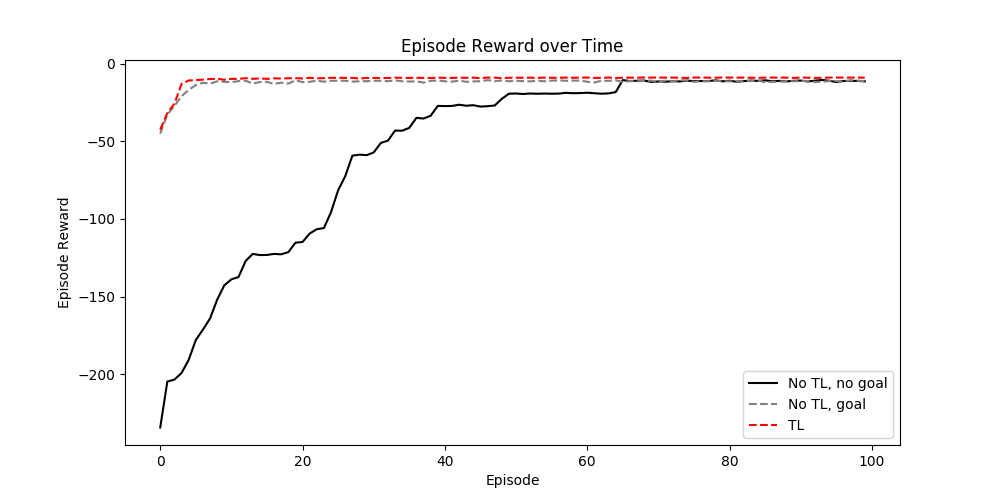
\includegraphics[width=0.55\textwidth]{./figures/experiment3_after_training}
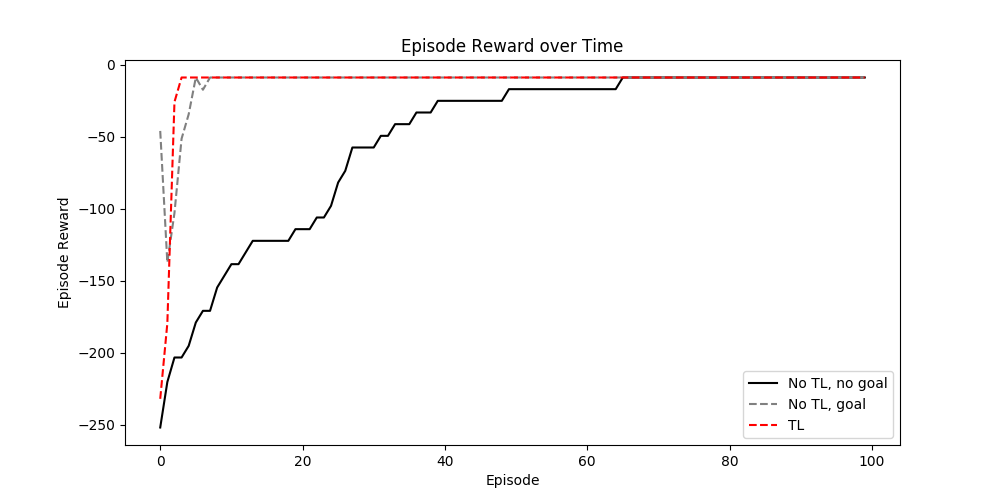
\includegraphics[width=0.55\textwidth]{./figures/experiment3_after_test}
}
\caption{Results of experiment 3: learning curve (left) and testing (right)}
\label{experiment3_training}
\end{figure}


\subsection{Experiment 4: Setup}
\label{subsec:experiement4_setup}
\begin{figure}[!htb]
\centerline{
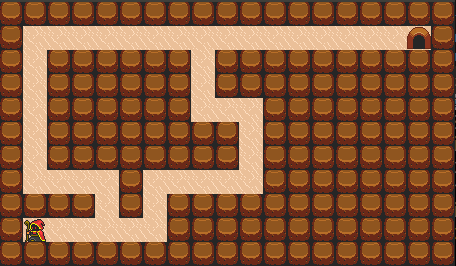
\includegraphics[width=0.5\textwidth]{./figures/experiment4_before}
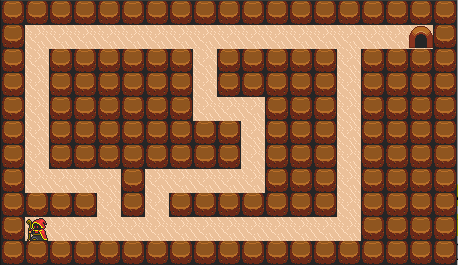
\includegraphics[width=0.5\textwidth]{./figures/experiment4_after}}
\caption{Game environment for experiment 4: before (left) and after (right) transfer learning}
\label{experiment4_setup}
\end{figure}

The transferred hypotheses are the same as that in Experiment 3, and the positive examples were collected the environment on the left in Figure \ref{experiment4_setup}.
The new environment, shown on the right in Figure \ref{experiment4_setup}, is the same except that there is teleport links.
This is a new concept that did not exist in the trained environment and therefore the agent needs to learn it after the hypothesis is transferred.
The same as Experiment 3, we use four different agents.

\subsection{Experiment Result 4}
\label{subsec:experiment_result_4}

Figure \ref{experiment4_training_test} show the results of the performance. The agent is able to succeffully learn the new concept and quickly finds the optimal policy at the early episodes.
This confirms that the transferred agents learns on top of what is already learnt. This experiment shows that the hypotheses is transferable even in cases where there is something the agent needs to learn in a new environment.

Also the difference of the state where the link is located does not cause any problems even when the positive examples in the previous environment is transferred, since the surrounding information is within the context rather than background knowledge. 
This shows the power of context dependent examples in RL senarios.

\begin{figure}[!htb]
\centerline{
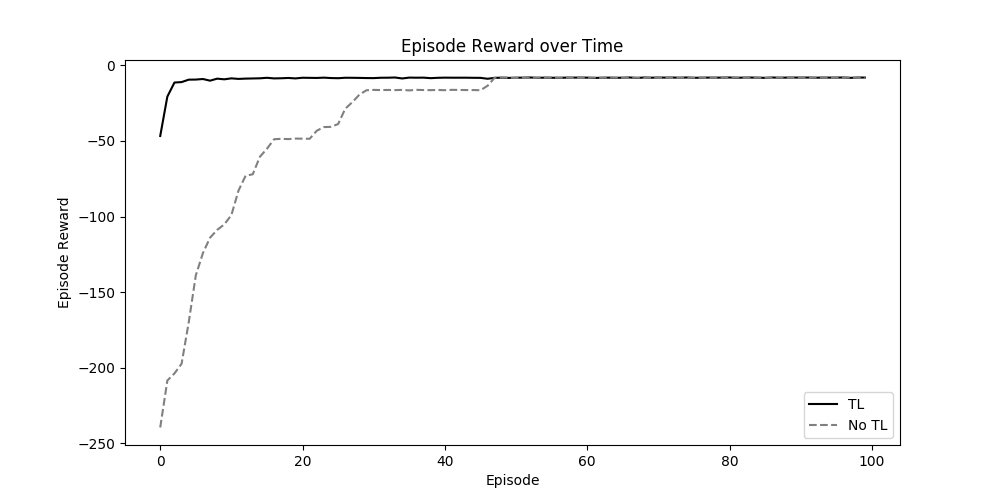
\includegraphics[width=0.55\textwidth]{./figures/experiment4_training}
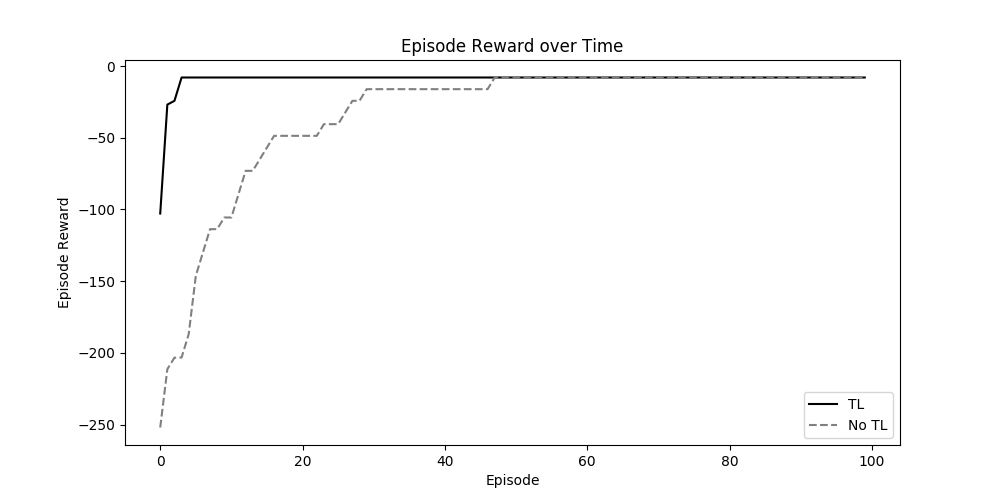
\includegraphics[width=0.55\textwidth]{./figures/experiment4_test}
}
\caption{Result of experiment 4 (learning curve)}
\label{experiment4_training_test}
\end{figure}

The new hypotheses the agent learns are the same as that of Experiment 2. The hypothesis containing \textsf{link\_start} and \textsf{link\_dest} is what the agent learnt in the new environment.

\lstinputlisting[
%   language = Prolog,
  caption  = {Hypotheses for experiment 4},
]{experiment4_hypothesis.pl}

\clearpage

\section{Discussion}
\label{sec:discussion}

We investigaged the properties of ILP(RL) using a simple maze environment. While the development of ILP(RL) is still in early stage and only a proof-of-concept, 
we observe both strengths as well as weakness of the current approach. We summarise both of these in the following sections.

\subsection{Strengths of ILP(RL)}
on a simple maze environment, which is the main target of our framework.

Although this is the first time and inductive logic programming is applied into reinforcement leaning and there are new interesting property for ILP(RL),
there are two major limitations with the current framework.

\begin{description}
\item[Faster learning convergence]
The agent with ILP(RL) learns the valid move of the environment at the very early stage of learning and, as soon as it finds the terminal state, is able to genrate a plan as a sequence of actions to reach the goal.
While this is a proof-of-concept approach, this way of RL is a new and the experiments show that this is a promissing direction of the research.

\item[Transfer Learning]
Unlike existing RL algorithms, where it learns value functions ro Q values, ILP(RL) learns a valid move as a hypotheses, which can be applied to similar but different environments.
We confimed with the experiments and, especially when the goal is known to the agent
We also show that the agent can learn a new hypothesis on top of the transferred ones, which is very flexible in terms of applicability of the learnt hypotheses.

\item[Symbolic learning]
Since both planning and learning can be expressed in ASP syntax, the learning process is easy to understand for human users, and the learnt hypotheses are a very general rule of the game.

In simple environments, we show that the agent learns rule of the game faster than existing RL algorithms, learnt concepts is easy to understand for human users.
\end{description} 

% The full hypotheses were learnt in the very early phase of learning and exploration phase. Thus with sufficient exploration, the model of the environment is correct
% and therefore it is able to find the optimal policy/path. 

% We show that ILP(RL) is able to solve a reduced MDP where the rewards are assumed to be associated with a sequence of actions planned as answer sets.
% Although this is a limitated solution, there is a potential to expand it to solve full MDP as discussed in Further Research. 

\subsection{Limitations of the current framework}
\label{subsec:limitations}
Although the this first version of the ILP(RL) framework using ILASP and ASP show potentials, there are a number of limitations with the current frameworks.
Some of these limitations are further elaborated in Further Research in the concluding chapter.

It was implement from scratch.

\begin{description}
\item[Learning time]
While we show that ILP(RL) improves the learning convergence in terms of the number of episodes required, the computational time is significantly longer than that of benchmarks due to the computation required for inductive learning with ILASP.
This limitation indicates that ILP(RL) may not be suitable in an environment where there is a moving object based on time rather than time steps.

Unlike existing reinforcement learning,
out algorithm refines hypothesis at every time steps within the same episode.
Thus even though the efficiency in terms of the number of iteration is higher,
training time within each iteration tends to be lower.

\item[Scalability issue for more complex environment]
ILP framework is known to be less scalable. The current framework is tested in a relatively simple environments, 
and proven to be work better than RL algorithsm in terms of the number of episodes that is needed to converge to an optimal policy.
However, learning in each episode is relatively slower than that of RL. 
This is shown in XXX, which shows average learnint time for ILASP. 

This limitation is theoretically discussed in XXX, where the complexity of deciding satisfiability is 
As shown in Experiment 1 and Experiment 2, adding two language bias significantly increased the runtime of the algorithm, since the search space grows significantly with respect to the language bias.

$\sum_{2}^{P}$-complete. Since there is no negative examples used in our current framework, the complexity is NP-complete.

Whereas Q-learning update value function in the same way whether there is a new concept such as teleport links.

Another question remains to how to extend the framework to more realistic senarios. RL works in more complex environments such as 3D or real physical environment, 
whereas the experiences of the agent in the current framework need to be expressed as ASP syntax, thus expressing continuous states rather than discrete states is challenging.

\item[Requirements of assumptions]

Language bias
While most of existing reinforcement learning works in different kinds of environment without pre-configuration, our algorithm
needs to define search space for learning hypothesis. As explained in the experiment 3, it was necessary to add two extra modeb before training.
Thus the algorithm may not be feasible in cases where these learning concepts were unknown or difficult to define with language bias. 

In addition, not only it needs search space, surrounding information is assumed to be known to the agent. 
While this assumption may be reasonable in many cases, this is not common in traditional reinforcement learning setting.

\item[limited MDP]
The current framework does not make use of rewards the agent collects and mainly uses the location of the goal for planning.
In some senarios, there may not be a termination state (goal) and instead there may be a different purpose to gain these rewards. 
Since the current implementation is dependent on finding the goal for planning rather than maximing total rewards, which is the common objective for most of RL algorithms,
the application of the current framework may be limited to particular types of problems.

There are some promissing solutions for some of these limitations, which we discuss in the next chapter.

\end{description}  

